% Created by tikzDevice version 0.12.6 on 2026-08-03 04:28:44
% !TEX encoding = UTF-8 Unicode
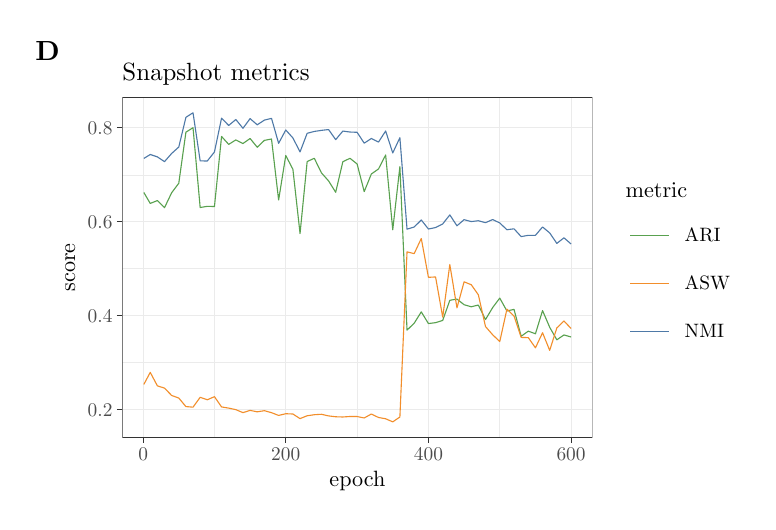
\begin{tikzpicture}[x=1pt,y=1pt]
\definecolor{fillColor}{RGB}{255,255,255}
\path[use as bounding box,fill=fillColor,fill opacity=0.00] (0,0) rectangle (260.22,171.36);
\begin{scope}
\path[clip] (  0.79,  1.87) rectangle (259.43,169.49);
\definecolor{drawColor}{RGB}{255,255,255}
\definecolor{fillColor}{RGB}{255,255,255}

\path[draw=drawColor,line width= 0.4pt,line join=round,line cap=round,fill=fillColor] (  0.79,  1.87) rectangle (259.43,169.49);
\end{scope}
\begin{scope}
\path[clip] ( 34.25, 23.34) rectangle (204.08,146.20);
\definecolor{fillColor}{RGB}{255,255,255}

\path[fill=fillColor] ( 34.25, 23.34) rectangle (204.08,146.20);
\definecolor{drawColor}{gray}{0.92}

\path[draw=drawColor,line width= 0.2pt,line join=round] ( 34.25, 50.36) --
	(204.08, 50.36);

\path[draw=drawColor,line width= 0.2pt,line join=round] ( 34.25, 84.27) --
	(204.08, 84.27);

\path[draw=drawColor,line width= 0.2pt,line join=round] ( 34.25,118.18) --
	(204.08,118.18);

\path[draw=drawColor,line width= 0.2pt,line join=round] ( 67.49, 23.34) --
	( 67.49,146.20);

\path[draw=drawColor,line width= 0.2pt,line join=round] (119.04, 23.34) --
	(119.04,146.20);

\path[draw=drawColor,line width= 0.2pt,line join=round] (170.59, 23.34) --
	(170.59,146.20);

\path[draw=drawColor,line width= 0.4pt,line join=round] ( 34.25, 33.41) --
	(204.08, 33.41);

\path[draw=drawColor,line width= 0.4pt,line join=round] ( 34.25, 67.32) --
	(204.08, 67.32);

\path[draw=drawColor,line width= 0.4pt,line join=round] ( 34.25,101.22) --
	(204.08,101.22);

\path[draw=drawColor,line width= 0.4pt,line join=round] ( 34.25,135.13) --
	(204.08,135.13);

\path[draw=drawColor,line width= 0.4pt,line join=round] ( 41.71, 23.34) --
	( 41.71,146.20);

\path[draw=drawColor,line width= 0.4pt,line join=round] ( 93.26, 23.34) --
	( 93.26,146.20);

\path[draw=drawColor,line width= 0.4pt,line join=round] (144.81, 23.34) --
	(144.81,146.20);

\path[draw=drawColor,line width= 0.4pt,line join=round] (196.36, 23.34) --
	(196.36,146.20);
\definecolor{drawColor}{RGB}{89,161,79}

\path[draw=drawColor,line width= 0.4pt,line join=round] ( 41.97,111.81) --
	( 44.29,107.84) --
	( 46.87,108.89) --
	( 49.44,106.30) --
	( 52.02,111.69) --
	( 54.60,115.14) --
	( 57.18,133.59) --
	( 59.75,135.22) --
	( 62.33,106.37) --
	( 64.91,106.80) --
	( 67.49,106.73) --
	( 70.06,132.04) --
	( 72.64,129.19) --
	( 75.22,130.80) --
	( 77.80,129.49) --
	( 80.37,131.32) --
	( 82.95,128.15) --
	( 85.53,130.63) --
	( 88.11,131.13) --
	( 90.68,109.08) --
	( 93.26,125.16) --
	( 95.84,120.19) --
	( 98.42, 96.97) --
	(100.99,122.98) --
	(103.57,124.17) --
	(106.15,118.89) --
	(108.73,115.99) --
	(111.30,111.88) --
	(113.88,122.90) --
	(116.46,124.16) --
	(119.04,122.11) --
	(121.61,112.12) --
	(124.19,118.49) --
	(126.77,120.30) --
	(129.35,125.35) --
	(131.92, 98.34) --
	(134.50,121.17) --
	(137.08, 62.07) --
	(139.66, 64.56) --
	(142.23, 68.66) --
	(144.81, 64.44) --
	(147.39, 64.76) --
	(149.97, 65.57) --
	(152.54, 72.84) --
	(155.12, 73.30) --
	(157.70, 71.25) --
	(160.28, 70.51) --
	(162.85, 71.13) --
	(165.43, 65.89) --
	(168.01, 70.20) --
	(170.59, 73.64) --
	(173.17, 68.99) --
	(175.74, 69.56) --
	(178.32, 59.85) --
	(180.90, 61.69) --
	(183.48, 60.75) --
	(186.05, 69.13) --
	(188.63, 63.10) --
	(191.21, 58.57) --
	(193.79, 60.32) --
	(196.36, 59.59);
\definecolor{drawColor}{RGB}{242,142,43}

\path[draw=drawColor,line width= 0.4pt,line join=round] ( 41.97, 42.43) --
	( 44.29, 46.81) --
	( 46.87, 41.92) --
	( 49.44, 41.12) --
	( 52.02, 38.46) --
	( 54.60, 37.53) --
	( 57.18, 34.44) --
	( 59.75, 34.23) --
	( 62.33, 37.80) --
	( 64.91, 36.90) --
	( 67.49, 38.02) --
	( 70.06, 34.31) --
	( 72.64, 33.89) --
	( 75.22, 33.33) --
	( 77.80, 32.25) --
	( 80.37, 33.07) --
	( 82.95, 32.54) --
	( 85.53, 32.96) --
	( 88.11, 32.24) --
	( 90.68, 31.24) --
	( 93.26, 31.86) --
	( 95.84, 31.76) --
	( 98.42, 30.09) --
	(100.99, 31.12) --
	(103.57, 31.50) --
	(106.15, 31.66) --
	(108.73, 31.07) --
	(111.30, 30.76) --
	(113.88, 30.68) --
	(116.46, 30.86) --
	(119.04, 30.84) --
	(121.61, 30.33) --
	(124.19, 31.76) --
	(126.77, 30.50) --
	(129.35, 30.04) --
	(131.92, 28.92) --
	(134.50, 30.67) --
	(137.08, 90.36) --
	(139.66, 89.71) --
	(142.23, 95.17) --
	(144.81, 81.15) --
	(147.39, 81.28) --
	(149.97, 66.78) --
	(152.54, 85.77) --
	(155.12, 70.11) --
	(157.70, 79.52) --
	(160.28, 78.48) --
	(162.85, 74.84) --
	(165.43, 63.37) --
	(168.01, 60.40) --
	(170.59, 57.94) --
	(173.17, 69.63) --
	(175.74, 67.16) --
	(178.32, 59.43) --
	(180.90, 59.36) --
	(183.48, 55.67) --
	(186.05, 61.12) --
	(188.63, 54.75) --
	(191.21, 62.86) --
	(193.79, 65.37) --
	(196.36, 62.65);
\definecolor{drawColor}{RGB}{78,121,167}

\path[draw=drawColor,line width= 0.4pt,line join=round] ( 41.97,124.10) --
	( 44.29,125.53) --
	( 46.87,124.67) --
	( 49.44,122.94) --
	( 52.02,125.90) --
	( 54.60,128.22) --
	( 57.18,138.97) --
	( 59.75,140.61) --
	( 62.33,123.21) --
	( 64.91,123.19) --
	( 67.49,126.44) --
	( 70.06,138.67) --
	( 72.64,136.02) --
	( 75.22,138.17) --
	( 77.80,135.00) --
	( 80.37,138.50) --
	( 82.95,136.25) --
	( 85.53,137.96) --
	( 88.11,138.58) --
	( 90.68,129.57) --
	( 93.26,134.38) --
	( 95.84,131.51) --
	( 98.42,126.47) --
	(100.99,133.19) --
	(103.57,133.86) --
	(106.15,134.25) --
	(108.73,134.54) --
	(111.30,130.90) --
	(113.88,133.99) --
	(116.46,133.65) --
	(119.04,133.55) --
	(121.61,129.62) --
	(124.19,131.33) --
	(126.77,130.02) --
	(129.35,134.02) --
	(131.92,126.09) --
	(134.50,131.61) --
	(137.08, 98.54) --
	(139.66, 99.33) --
	(142.23,101.87) --
	(144.81, 98.60) --
	(147.39, 99.13) --
	(149.97,100.45) --
	(152.54,103.70) --
	(155.12, 99.77) --
	(157.70,101.98) --
	(160.28,101.29) --
	(162.85,101.60) --
	(165.43,100.89) --
	(168.01,102.02) --
	(170.59,100.80) --
	(173.17, 98.34) --
	(175.74, 98.68) --
	(178.32, 95.86) --
	(180.90, 96.33) --
	(183.48, 96.32) --
	(186.05, 99.35) --
	(188.63, 97.19) --
	(191.21, 93.41) --
	(193.79, 95.42) --
	(196.36, 93.19);
\definecolor{drawColor}{gray}{0.20}

\path[draw=drawColor,line width= 0.4pt,line join=round,line cap=round] ( 34.25, 23.34) rectangle (204.08,146.20);
\end{scope}
\begin{scope}
\path[clip] (  0.00,  0.00) rectangle (260.22,171.36);
\definecolor{drawColor}{gray}{0.30}

\node[text=drawColor,anchor=base east,inner sep=0pt, outer sep=0pt, scale=  0.70] at ( 30.65, 31.00) {0.2};

\node[text=drawColor,anchor=base east,inner sep=0pt, outer sep=0pt, scale=  0.70] at ( 30.65, 64.91) {0.4};

\node[text=drawColor,anchor=base east,inner sep=0pt, outer sep=0pt, scale=  0.70] at ( 30.65, 98.81) {0.6};

\node[text=drawColor,anchor=base east,inner sep=0pt, outer sep=0pt, scale=  0.70] at ( 30.65,132.72) {0.8};
\end{scope}
\begin{scope}
\path[clip] (  0.00,  0.00) rectangle (260.22,171.36);
\definecolor{drawColor}{gray}{0.20}

\path[draw=drawColor,line width= 0.4pt,line join=round] ( 32.25, 33.41) --
	( 34.25, 33.41);

\path[draw=drawColor,line width= 0.4pt,line join=round] ( 32.25, 67.32) --
	( 34.25, 67.32);

\path[draw=drawColor,line width= 0.4pt,line join=round] ( 32.25,101.22) --
	( 34.25,101.22);

\path[draw=drawColor,line width= 0.4pt,line join=round] ( 32.25,135.13) --
	( 34.25,135.13);
\end{scope}
\begin{scope}
\path[clip] (  0.00,  0.00) rectangle (260.22,171.36);
\definecolor{drawColor}{gray}{0.20}

\path[draw=drawColor,line width= 0.4pt,line join=round] ( 41.71, 21.34) --
	( 41.71, 23.34);

\path[draw=drawColor,line width= 0.4pt,line join=round] ( 93.26, 21.34) --
	( 93.26, 23.34);

\path[draw=drawColor,line width= 0.4pt,line join=round] (144.81, 21.34) --
	(144.81, 23.34);

\path[draw=drawColor,line width= 0.4pt,line join=round] (196.36, 21.34) --
	(196.36, 23.34);
\end{scope}
\begin{scope}
\path[clip] (  0.00,  0.00) rectangle (260.22,171.36);
\definecolor{drawColor}{gray}{0.30}

\node[text=drawColor,anchor=base,inner sep=0pt, outer sep=0pt, scale=  0.70] at ( 41.71, 14.92) {0};

\node[text=drawColor,anchor=base,inner sep=0pt, outer sep=0pt, scale=  0.70] at ( 93.26, 14.92) {200};

\node[text=drawColor,anchor=base,inner sep=0pt, outer sep=0pt, scale=  0.70] at (144.81, 14.92) {400};

\node[text=drawColor,anchor=base,inner sep=0pt, outer sep=0pt, scale=  0.70] at (196.36, 14.92) {600};
\end{scope}
\begin{scope}
\path[clip] (  0.00,  0.00) rectangle (260.22,171.36);
\definecolor{drawColor}{RGB}{0,0,0}

\node[text=drawColor,anchor=base,inner sep=0pt, outer sep=0pt, scale=  0.80] at (119.17,  5.64) {epoch};
\end{scope}
\begin{scope}
\path[clip] (  0.00,  0.00) rectangle (260.22,171.36);
\definecolor{drawColor}{RGB}{0,0,0}

\node[text=drawColor,rotate= 90.00,anchor=base,inner sep=0pt, outer sep=0pt, scale=  0.80] at ( 17.12, 84.77) {score};
\end{scope}
\begin{scope}
\path[clip] (  0.00,  0.00) rectangle (260.22,171.36);
\definecolor{fillColor}{RGB}{255,255,255}

\path[fill=fillColor] (212.08, 48.98) rectangle (257.43,120.55);
\end{scope}
\begin{scope}
\path[clip] (  0.00,  0.00) rectangle (260.22,171.36);
\definecolor{drawColor}{RGB}{0,0,0}

\node[text=drawColor,anchor=base west,inner sep=0pt, outer sep=0pt, scale=  0.80] at (216.08,110.03) {metric};
\end{scope}
\begin{scope}
\path[clip] (  0.00,  0.00) rectangle (260.22,171.36);
\definecolor{fillColor}{RGB}{255,255,255}

\path[fill=fillColor] (216.08, 87.67) rectangle (233.43,105.02);
\definecolor{drawColor}{RGB}{89,161,79}

\path[draw=drawColor,line width= 0.4pt,line join=round] (217.82, 96.35) -- (231.69, 96.35);
\end{scope}
\begin{scope}
\path[clip] (  0.00,  0.00) rectangle (260.22,171.36);
\definecolor{fillColor}{RGB}{255,255,255}

\path[fill=fillColor] (216.08, 70.33) rectangle (233.43, 87.67);
\definecolor{drawColor}{RGB}{242,142,43}

\path[draw=drawColor,line width= 0.4pt,line join=round] (217.82, 79.00) -- (231.69, 79.00);
\end{scope}
\begin{scope}
\path[clip] (  0.00,  0.00) rectangle (260.22,171.36);
\definecolor{fillColor}{RGB}{255,255,255}

\path[fill=fillColor] (216.08, 52.98) rectangle (233.43, 70.33);
\definecolor{drawColor}{RGB}{78,121,167}

\path[draw=drawColor,line width= 0.4pt,line join=round] (217.82, 61.66) -- (231.69, 61.66);
\end{scope}
\begin{scope}
\path[clip] (  0.00,  0.00) rectangle (260.22,171.36);
\definecolor{drawColor}{RGB}{0,0,0}

\node[text=drawColor,anchor=base west,inner sep=0pt, outer sep=0pt, scale=  0.70] at (237.43, 93.93) {ARI};
\end{scope}
\begin{scope}
\path[clip] (  0.00,  0.00) rectangle (260.22,171.36);
\definecolor{drawColor}{RGB}{0,0,0}

\node[text=drawColor,anchor=base west,inner sep=0pt, outer sep=0pt, scale=  0.70] at (237.43, 76.59) {ASW};
\end{scope}
\begin{scope}
\path[clip] (  0.00,  0.00) rectangle (260.22,171.36);
\definecolor{drawColor}{RGB}{0,0,0}

\node[text=drawColor,anchor=base west,inner sep=0pt, outer sep=0pt, scale=  0.70] at (237.43, 59.25) {NMI};
\end{scope}
\begin{scope}
\path[clip] (  0.00,  0.00) rectangle (260.22,171.36);
\definecolor{drawColor}{RGB}{0,0,0}

\node[text=drawColor,anchor=base west,inner sep=0pt, outer sep=0pt, scale=  0.90] at ( 34.25,152.18) {Snapshot metrics};
\end{scope}
\begin{scope}
\path[clip] (  0.00,  0.00) rectangle (260.22,171.36);
\definecolor{drawColor}{RGB}{0,0,0}

\node[text=drawColor,anchor=base,inner sep=0pt, outer sep=0pt, scale=  1.00] at (  7.20,159.49) {\bfseries D};
\end{scope}
\end{tikzpicture}
